\documentclass[man,floatsintext]{apa6}
\usepackage{lmodern}
\usepackage{amssymb,amsmath}
\usepackage{ifxetex,ifluatex}
\usepackage{fixltx2e} % provides \textsubscript
\ifnum 0\ifxetex 1\fi\ifluatex 1\fi=0 % if pdftex
  \usepackage[T1]{fontenc}
  \usepackage[utf8]{inputenc}
\else % if luatex or xelatex
  \ifxetex
    \usepackage{mathspec}
  \else
    \usepackage{fontspec}
  \fi
  \defaultfontfeatures{Ligatures=TeX,Scale=MatchLowercase}
\fi
% use upquote if available, for straight quotes in verbatim environments
\IfFileExists{upquote.sty}{\usepackage{upquote}}{}
% use microtype if available
\IfFileExists{microtype.sty}{%
\usepackage{microtype}
\UseMicrotypeSet[protrusion]{basicmath} % disable protrusion for tt fonts
}{}
\usepackage{hyperref}
\hypersetup{unicode=true,
            pdftitle={On Gravitation and Learning},
            pdfauthor={Andrei Amatuni~\& Barack Obama},
            pdfkeywords={word learning, gravity, development, complex systems},
            pdfborder={0 0 0},
            breaklinks=true}
\urlstyle{same}  % don't use monospace font for urls
\usepackage{graphicx,grffile}
\makeatletter
\def\maxwidth{\ifdim\Gin@nat@width>\linewidth\linewidth\else\Gin@nat@width\fi}
\def\maxheight{\ifdim\Gin@nat@height>\textheight\textheight\else\Gin@nat@height\fi}
\makeatother
% Scale images if necessary, so that they will not overflow the page
% margins by default, and it is still possible to overwrite the defaults
% using explicit options in \includegraphics[width, height, ...]{}
\setkeys{Gin}{width=\maxwidth,height=\maxheight,keepaspectratio}
\IfFileExists{parskip.sty}{%
\usepackage{parskip}
}{% else
\setlength{\parindent}{0pt}
\setlength{\parskip}{6pt plus 2pt minus 1pt}
}
\setlength{\emergencystretch}{3em}  % prevent overfull lines
\providecommand{\tightlist}{%
  \setlength{\itemsep}{0pt}\setlength{\parskip}{0pt}}
\setcounter{secnumdepth}{0}
% Redefines (sub)paragraphs to behave more like sections
\ifx\paragraph\undefined\else
\let\oldparagraph\paragraph
\renewcommand{\paragraph}[1]{\oldparagraph{#1}\mbox{}}
\fi
\ifx\subparagraph\undefined\else
\let\oldsubparagraph\subparagraph
\renewcommand{\subparagraph}[1]{\oldsubparagraph{#1}\mbox{}}
\fi

%%% Use protect on footnotes to avoid problems with footnotes in titles
\let\rmarkdownfootnote\footnote%
\def\footnote{\protect\rmarkdownfootnote}


  \title{On Gravitation and Learning}
    \author{Andrei Amatuni\textsuperscript{1}~\& Barack Obama\textsuperscript{1,2}}
    \date{}
  
\shorttitle{Gravity and Learning}
\affiliation{
\vspace{0.5cm}
\textsuperscript{1} Indiana University\\\textsuperscript{2} University of Chicago}
\keywords{word learning, gravity, development, complex systems\newline\indent Word count: X}
\usepackage{csquotes}
\usepackage{upgreek}
\captionsetup{font=singlespacing,justification=justified}

\usepackage{longtable}
\usepackage{lscape}
\usepackage{multirow}
\usepackage{tabularx}
\usepackage[flushleft]{threeparttable}
\usepackage{threeparttablex}

\newenvironment{lltable}{\begin{landscape}\begin{center}\begin{ThreePartTable}}{\end{ThreePartTable}\end{center}\end{landscape}}

\makeatletter
\newcommand\LastLTentrywidth{1em}
\newlength\longtablewidth
\setlength{\longtablewidth}{1in}
\newcommand{\getlongtablewidth}{\begingroup \ifcsname LT@\roman{LT@tables}\endcsname \global\longtablewidth=0pt \renewcommand{\LT@entry}[2]{\global\advance\longtablewidth by ##2\relax\gdef\LastLTentrywidth{##2}}\@nameuse{LT@\roman{LT@tables}} \fi \endgroup}


\usepackage{lineno}

\linenumbers

\authornote{Add complete departmental affiliations for each author here. Each new line herein must be indented, like this line.

Enter author note here.

Correspondence concerning this article should be addressed to Andrei Amatuni, 332 Reindeer Lane, North Pole, Arctic Circle. E-mail: \href{mailto:andrei.amatuni@gmail.com}{\nolinkurl{andrei.amatuni@gmail.com}}}

\abstract{
Here we study the relationship between gravitation and learning in young infants. We demonstrate a significant correspondence between the mass of a learning agent and their ability to learn in a series of novel word learning experiments. This has far reaching consequences for our understanding of development and the nature of intelligence and time.


}

\begin{document}
\maketitle

\hypertarget{introduction}{%
\section{Introduction}\label{introduction}}

Here you're gonna want to start talking about what your paper is about and why someone should keep reading beyond the first sentence. You want to make it juicey and intruiguing, but careful, if there's too much juice the reader might drown.

\hypertarget{on-the-nature-of-time}{%
\section{On the Nature of Time}\label{on-the-nature-of-time}}

Now that the reader is fully invested in your work and the questions that it's going to be tackling, you can start getting deep into the weeds and explain things in excruciating detail. If you want to throw some math in the mix, you do that by surrounding LaTex math expressions with \$ signs, where in-line expressions like \(2 + 2 = 4\) use only one dollar sign, and if you want an expression to be on it's own line, you surround the expression with two \$ signs, like so: \[\zeta(s) = \sum_{n=1}^{\infty} \frac{1}{n^s}\]

You're probably going to want to cite some people so that your reader doesn't feel like you're pulling all this stuff out of nowhere, make them feel like other humans have thought in similar directions and the broader scientific community considered their inquiries worthy of publication. To cite someone, you add a @ symbol before the bibtex entry title and surround that in square brackets like so (Sigman \& Cecchi, 2002). If you want to cite multiple people at once in one instance, you do the same thing, but separate each paper with a semi-colon like so (Hills, Maouene, Riordan, \& Smith, 2010; Hills, Maouene, Maouene, Sheya, \& Smith, 2009; Steyvers \& Tenenbaum, 2005). When you leave the square brackets out, then the citation becomes an in-text citation, which is useful if you want the names of the authors to be part of the flow of your prose, like if I want to say that Goodman, Dale, and Li (2008) did some cool work and the reader should know about it.

\hypertarget{methods}{%
\section{Methods}\label{methods}}

Now that you're past all the initial fluff of the paper, it's time to get down to brass tacks. What did you actually do? Let the reader know what's up.

\hypertarget{study-1-measuring-the-gravitational-interaction-of-learning-bodies}{%
\subsection{Study 1: Measuring the Gravitational Interaction of Learning Bodies}\label{study-1-measuring-the-gravitational-interaction-of-learning-bodies}}

Note that you can create sub-sub-sub-etc headings by adding more and more \# signs. For the first study, we weighted different children, and then exposed them to a bunch of word/object pairings, and then tested how many novel words they learned at the end of training.

\hypertarget{results}{%
\subsubsection{Results}\label{results}}

You're probably going to need to load the actual data that has all your results. You need to do this within R blocks, which you can insert with the shortcut option+command+I on Mac and ctrl+alt+I on Windows

You can do this data loading at any point in the document (except in the header), so you could have loaded all the libraries and data at the very beginning, or wherever.

Now you'll probably want to visualize the data you loaded, which is where ggplot comes in. This is the defacto standard library for plotting in R. You'll notice that at the very beginning of the article we imported a library called \enquote{tidyverse}. This is where ggplot and a bunch of other really powerful R packages live. If you want to be a data wrangling and visualization wizard, learn tidyverse\(\footnote{\texttt{https://r4ds.had.co.nz/}}\)

\begin{figure}
\centering
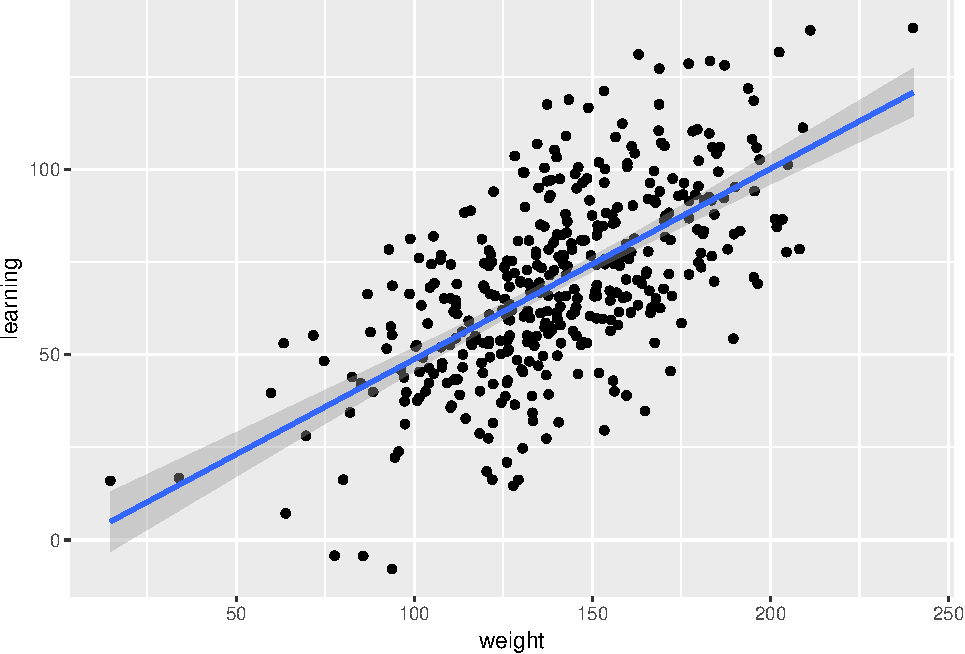
\includegraphics{tutorial_files/figure-latex/weight-and-learning-1.pdf}
\caption{\label{fig:weight-and-learning}This is where you add the figure caption. You can also add information about the statistics that}
\end{figure}

To insert a plot that's defined within an R chunk, you'll need to refer to is within your text. So you'll need to say something like, see Figure \ref{fig:weight-and-learning}. By default the papaja package will put these figures at the end, as that's what APA expects, but you can tell it to put the figures within the text by setting the \enquote{floatsintext} parameter to \enquote{yes}.

Woah. It looks like the more mass that a organism has, the better they learn. Let's look at another plot that groups points by some categorical variable and tiles plots according to this grouping.

\begin{figure}
\centering
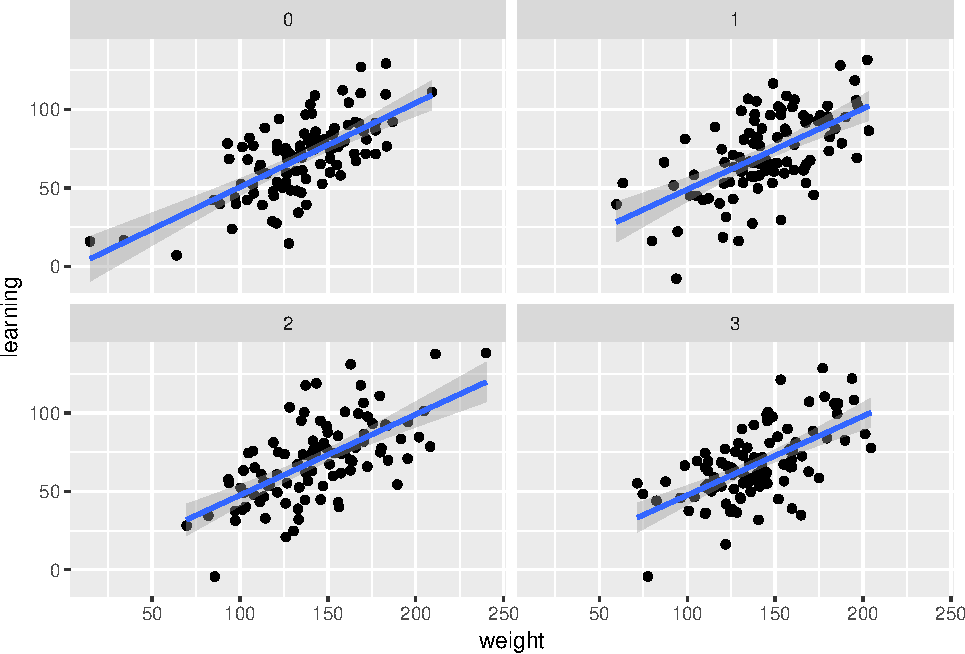
\includegraphics{tutorial_files/figure-latex/tiled-weight-1.pdf}
\caption{\label{fig:tiled-weight}This is the same data as in the previous plot, except points have been grouped by what experiment they were in, where experiments are numbered 1-4.}
\end{figure}

\newpage

\hypertarget{references}{%
\section{References}\label{references}}

\begingroup
\setlength{\parindent}{-0.5in}
\setlength{\leftskip}{0.5in}

\hypertarget{refs}{}
\leavevmode\hypertarget{ref-goodman2008frequency}{}%
Goodman, J. C., Dale, P. S., \& Li, P. (2008). Does frequency count? Parental input and the acquisition of vocabulary. \emph{Journal of Child Language}, \emph{35}(03), 515--531.

\leavevmode\hypertarget{ref-hills2010associative}{}%
Hills, T. T., Maouene, J., Riordan, B., \& Smith, L. B. (2010). The associative structure of language: Contextual diversity in early word learning. \emph{Journal of Memory and Language}, \emph{63}(3), 259--273.

\leavevmode\hypertarget{ref-hills2009longitudinal}{}%
Hills, T. T., Maouene, M., Maouene, J., Sheya, A., \& Smith, L. (2009). Longitudinal analysis of early semantic networks preferential attachment or preferential acquisition? \emph{Psychological Science}, \emph{20}(6), 729--739.

\leavevmode\hypertarget{ref-sigman2002global}{}%
Sigman, M., \& Cecchi, G. A. (2002). Global organization of the wordnet lexicon. \emph{Proceedings of the National Academy of Sciences}, \emph{99}(3), 1742--1747.

\leavevmode\hypertarget{ref-tenenbaum2005large}{}%
Steyvers, M., \& Tenenbaum, J. B. (2005). The large-scale structure of semantic networks: Statistical analyses and a model of semantic growth. \emph{Cognitive Science}, \emph{29}(1), 41--78.

\endgroup


\end{document}
